\documentclass[10pt,a4paper]{article}
\usepackage{graphicx}
\usepackage{placeins}
\usepackage{indentfirst}
\usepackage{enumitem}
\author{Bardi Bogdan}
\title{Polynomial Calculator}


\begin{document}
\begin{titlepage}
\centering

\includegraphics[width=0.5\paperwidth]{utcn.png}\par\vspace{5cm}
	{\huge\bfseries Queues Simulator\par}
	\vspace{2cm}
	{\Large\itshape Bardi Bogdan\par}
	{\Large\itshape Group:30421\par}
	{\Large\itshape Year of Study: 2019-2020\par}
	\vfill
\end{titlepage}
\tableofcontents
\pagebreak
\section{Requirements}
The main goal of this assignment was to design and implement a simulation application aiming to analyze queuing based systems for
determining and minimizing clients’ waiting time\par
To achieve the main objective I had to go through many different steps which will be thoroughly explained in the following chapters:
\begin{enumerate}
\item Analyzing use cases and the problem itself
\item Creating an UML Diagram and designing the necessary classes and data structures
\item Designing the user interface
\item Implementing the created designs
\item Creating unit tests
\end{enumerate}

\section{Problem Analysis}
Queues are commonly used to model real world domains. The main objective of a queue is to
provide a place for a "client" to wait before receiving a "service". The management of queue-based
system is interested in minimizing the time amount their "clients" are waiting in queues before
they are served. One way to minimize the waiting time is to add more servers, i.e. more queues in
the system (each queue is considered as having an associated processor) but this approach increases
the costs of the service supplier. When a new server is added the waiting customers will be evenly
distributed to all current available queues. \par
The application has to simulate a series of N clients arriving for service, entering Q queues, waiting, being served and finally leaving the queues. All clients are generated at the start of a simulation and have 3 characteristics: an ID(from 1 to N), t\textsubscript{simulation}(simulation time when the cilent goes to the queue, like when it finishes shopping), t\textsubscript{service}(the duration needed to serve the client by the cashier). The program will also keep track of the time spent by each client at the queues and compute the average waiting time after the simulation ends.\par
The necessary input data needed for the simulation are as follows:
\begin{itemize}
\item Number of clients(N)
\item Number of queues(Q)
\item Simulation interval(t\rlap{\textsuperscript{MAX}}\rlap{\textsubscript{simulation}}\space\space\space\space\space\space\space\space\space\space\space)
\item Minimum and maximum arrival time
\item Minimum and maximum service time
\end{itemize}
\pagebreak
The user will input the data into a text file which is passed as an application argument. The output of the application is a text file which contains the log of the simulation and the average waiting time of the clients.
\begin{figure}[!htb]

\centering
\includegraphics[scale=1]{a.mps}
\caption{Use case diagram}
\end{figure}

\section{Program Design}
In order to process the simulation efficiently a multi-threaded approach is used in order to leverage the multi-core capabilities of the processors. Each queue in the simulation has a thread allocated to it. Each thread has their own individual queue which is filled as clients come in by a Manager thread.\par
By definition, multitasking is when multiple processes share common processing resources such as a CPU. Multi-threading extends the idea of multitasking into applications where you can subdivide specific operations within a single application into individual threads. Each of the threads can run in parallel. The OS divides processing time not only among different applications, but also among each thread within an application.\par
The manager is responsible for handling the simulation time,distributing clients to the shortest queue and, managing each queue thread in order to ensure that a tick of the simulation has been processed by every server.It is also responsible with printing the output of the simulation.\par
Each queue thread is started when it receives a client and stopped when it runs out of clients to be processed in order to save processing resources.

UML, short for Unified Modeling Language, is a standardized modeling language consisting of an integrated set of diagrams, developed to help system and software developers for specifying, visualizing, constructing, and documenting the artifacts of software systems. It allows us to visualize the class structure of the three aforementioned packages and how they interact with each other.

\begin{figure}[!htb]
\centering
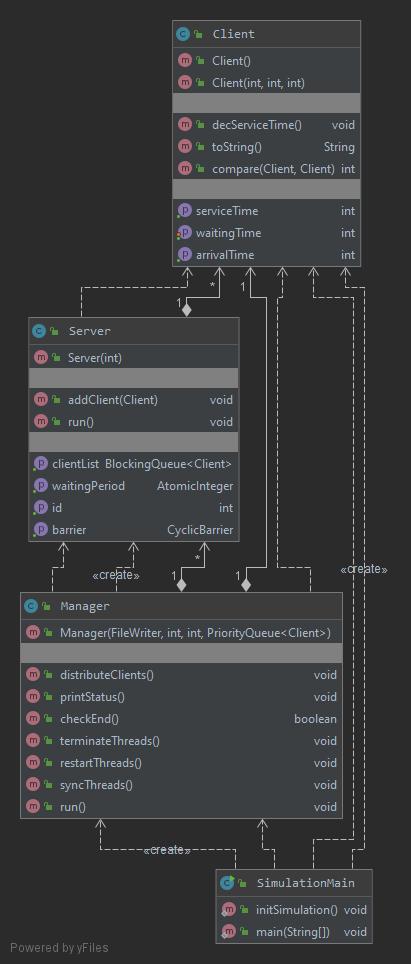
\includegraphics[scale=0.30]{package.png}
\caption{UML Diagram of the Model Package}
\end{figure}
\FloatBarrier
\section{Implementation}
\subsection{SimulationMain}
The SimulationMain class is responsible with fetching the program arguments and generating the list of clients according to the input data and then initializing the management thread.\par
The clients are generated randomly based on the time intervals given in the input text and then added to the queue.
\subsubsection{InitSimulation()}
The method generates the clients and creates an instance of the Manager class and starts its thread.
\subsubsection{main(String args[])}
The main of the application, is responsible with opening the files given in the arguments and reading the simulation parameters and calls InitSimulation()
\subsection{Manager}
The Manager class is responsible with printing the simulation output into a FileWriter, distributing the clients to their queues and keeping the time inside the simulation.It also is responsible with starting and restarting the Servers' coresponding threads when they get a new clients in their corresponding queue.
\subsubsection{Important Fields}
\begin{itemize}
\item generatedClients - queue of waiting clients
\item threadList - an ArrayList of threads for the queues
\item serversList - an ArrayList of the servers needed
\item outputWriter - an FileWriter to output to the external file given as an argument of the program
\item simulationTime - current time of the simulation(t\textsubscript{simulation})
\item finalTime - the maximum time allowed for the simulation(t\rlap{\textsuperscript{MAX}}\rlap{\textsubscript{simulation}}\space\space\space\space\space\space\space\space\space\space\space)
\item clientsServed - number of clients which were served by the servers
\item totalTimeSpent - tallies the amount of time the clients spent waiting at the queue
\end{itemize}
\subsubsection{Manager(outputWriter, finalTime, noOfServers, generatedClients)}
This constructor takes the FileWriter opened in the Main class, the simulation interval, number of queues and the generated Clients as a priority queue.Its main job is to initialize the important values, to instantiate the queues and prepares their threads for execution.
\subsubsection{distributeClients()}
This method will distribute will check for arrived clients (t\textsubscript{arrival}$\leq$ t\textsubscript{simulation}) and distribute them to their queues based on the minimum waiting time of the queues.
\subsubsection{checkEnd()}
This method will check if there are any more waiting clients or clients in their queues and will return a boolean truth value if so or a boolean false if not.
\subsubsection{terminateThreads()}
This method is called after ending the simulation to terminate any running client threads not finished yet in order to gracefully exit the program. It does so by first waiting for the tread to reach their barriers and then sending an interrupt signal. The raised exception will be caught by the run function of the thread and escape the running loop, allowing it to end.
\subsubsection{syncThreads()}
Method to allow for all running queue threads to reach either a waiting state or to terminate if they finish processing their final client 
\subsubsection{restartThreads()}
It (re)starts the threads corresponding to the recently filled queues.
\subsubsection{printStatus()}
It prints the state of the simulation at the time of calling it.
\subsubsection{run()}
The main body of the Manager thread. It makes use of all the auxiliary methods of the Management class to distribute clients,prints the step by step status of the simulation and synchronize the queue threads. It has a while loop which checks if the final time wasn't reached or if there aren't any more clients to process. Finally will terminate all remaining threads if there are any more.
\subsection{Server}
This class represents a queue server(i.e cashier), it implements the Runnable interface in order to be able to run its instances as separate threads.
\subsubsection{Important Fields}
\begin{itemize}
\item id - server id(useful for printing its state
\item clientList - a BlockingQueue(for thread safety) which stores the clients which are currently associated to this queue
\item waitingPeriod - an AtomicInteger which holds the current waiting period of the queue
\item managerBarrier - a CyclicBarrier which provides a handle for the manager to notify the thread of starting a new tick
\end{itemize}
\subsubsection{Server(int id)}
Class constructor which initializes the important fields with new instances of each and attributes the given id to its field
\subsubsection{getID()}
Returns the id of the server
\subsubsection{addClient(Client client)}
Adds a new client to the queue and updates the waiting period to reflect this change. The waiting period is calculated as such
waitingPeriod = waitingPeriod + client.servicePeriod.
\subsubsection{getClientList()}
It provides the queue of the server. Useful for printing it or checking if it is empty or not.
\subsubsection{getWaitingPerion()}
Fetches the current waiting period of the server.
\subsubsection{getBarrier()}
Fetches the barrier, needed for the manager to trip it
\subsubsection{run()}
The code run by the thread. At every run it will wait for the manager signal to start processing the tick and then will try to fetch the current client. If it manages to do so it will decrement its service time and decrement the current waiting period. If the client's service time reaches 0 it is removed from the queue. If the queue becomes empty then the thread terminates.
\subsection{Client}
It represents the actual client inside the simulation. It is generated by the SimulationMain and added to the queue in order to be processed.
\subsubsection{Important Fields}
\begin{itemize}
\item id - represents the client id
\item arrivalTime - the time of arrival
\item serviceTime - the time needed by the client to be serviced
\item waitingTime - the time waited by the client in order to receive the services needed	
\end{itemize}
\subsubsection{Client(id, arrivalTime, serviceTime)}
The constructor of the Client class which initializes the fields with the values given as arguments except for waiting time which is initialized with 0
\subsubsection{setWaitingTime(waitingTime)}
Sets the waiting time. It is usually called when the client is added to the queue to update the waiting time of the client
\subsubsection{compare(client,t1)}
Method inherited from the Comparator class, needed to create the priority queue sorted by the t\textsubscript{arrival}.
\section{Testing}
In the repository there are given three testing files and their corresponding results.
\subsection{in-test-1.txt}
This file simulates the conditions for a lightly occupied day, only 4 clients are spawned across 60 seconds of simulation and the chances of the queues being overloaded are low pretty much always finishing early depending on the randomly generated values. The waiting times are very low(close to the average of the service time)
\subsection{in-test-2.txt}
These are the conditions for a moderately occupied day, 50 clients divided among 5 queues will cause a fair amount of overloading the queues reaching at worst 3 clients waiting in line, but still won't reach the maximum time allocated for the simulation. The times are low (still close to the average of the service time)
\subsection{in-test-3.txt}
These are the conditions for a crowded day, 1000 clients divided among 20 queues, this will cause all the queues to be full with people and most of the time not even able to process everyone and the time will certainly run out. The waiting times are very high as the queues are overwhelmed by people and are unable to process them.
\section{Conclusions}
This assignment is a great introduction to Java multi-threading features. As it introduces us to the Runnable class, how to create threads in Java,different synchronization techniques and different synchronized data structures such as BlockingQueue and CountDownLatch.
\section{Bibliography}
\begin{itemize}
\item https://docs.oracle.com/javase/tutorial/essential/concurrency/index.html
\item https://www.baeldung.com/java-cyclic-barrier
\item https://www.tutorialspoint.com/java/java\_multithreading.htm
\item https://www.geeksforgeeks.org/generating-random-numbers-in-java/
\item B. Goetz et al., Java Concurrency in Practice, Addison-Wesley Professional; 1 edition (May 19, 2006)

\end{itemize}
\end{document}